\documentclass[dvips, lscape]{foils}
%\documentclass[dvips, french]{slides}
\textwidth 18.5cm
\textheight 25cm 
\topmargin -1cm 
\oddsidemargin  -1cm 
\evensidemargin  -1cm

% Maths
\usepackage{amsfonts, amsmath, amssymb}

\newcommand{\coefbin}[2]{\left( 
    \begin{array}{c} #1 \\ #2 \end{array} 
  \right)}
\newcommand{\bbullet}{\bullet\bullet}
\newcommand{\bbbullet}{\bbullet\bullet}
\newcommand{\bbbbullet}{\bbbullet\bullet}
\newcommand{\Bcal}{\mathcal{B}}
\newcommand{\Ccal}{\mathcal{C}}
\newcommand{\Dcal}{\mathcal{D}}
\newcommand{\Ecal}{\mathcal{E}}
\newcommand{\Mcal}{\mathcal{M}}
\newcommand{\Ncal}{\mathcal{N}}
\newcommand{\Pcal}{\mathcal{P}}
\newcommand{\Lcal}{\mathcal{L}}
\newcommand{\Tcal}{\mathcal{T}}
\newcommand{\Ucal}{\mathcal{U}}
\newcommand{\alphabf}{\mbox{\mathversion{bold}{$\alpha$}}}
\newcommand{\betabf}{\mbox{\mathversion{bold}{$\beta$}}}
\newcommand{\gammabf}{\mbox{\mathversion{bold}{$\gamma$}}}
\newcommand{\mubf}{\mbox{\mathversion{bold}{$\mu$}}}
\newcommand{\psibf}{\mbox{\mathversion{bold}{$\psi$}}}
\newcommand{\Sigmabf}{\mbox{\mathversion{bold}{$\Sigma$}}}
\newcommand{\taubf}{\mbox{\mathversion{bold}{$\tau$}}}
\newcommand{\thetabf}{\mbox{\mathversion{bold}{$\theta$}}}
\newcommand{\Dbf}{{\bf D}}
\newcommand{\Ebf}{{\bf E}}
\newcommand{\Hbf}{{\bf H}}
\newcommand{\Ibf}{{\bf I}}
\newcommand{\Sbf}{{\bf S}}
\newcommand{\mbf}{{\bf m}}
\newcommand{\ubf}{{\bf u}}
\newcommand{\vbf}{{\bf v}}
\newcommand{\xbf}{{\bf x}}
\newcommand{\Xbf}{{\bf X}}
\newcommand{\Esp}{{\mathbb E}}
\newcommand{\Corr}{{\mathbb C}\mbox{orr}}
\newcommand{\Var}{{\mathbb V}}
\newcommand{\Ibb}{{\mathbb I}}
\newcommand{\Rbb}{\mathbb{R}}

% Couleur et graphiques
\usepackage{color}
\usepackage{graphics}
\usepackage{epsfig} 
\usepackage{pstcol}

% Texte
\usepackage{lscape}
\usepackage{../../../../Latex/fancyheadings, rotating, enumerate}
%\usepackage[french]{babel}
\usepackage[latin1]{inputenc}
%\definecolor{darkgreen}{cmyk}{0.5, 0, 0.5, 0.5}
%\definecolor{green}{cmyk}{0.5, 0, 0.5, 0.5}
\definecolor{orange}{cmyk}{0, 0.6, 0.8, 0}
\definecolor{jaune}{cmyk}{0, 0.5, 0.5, 0}
\newcommand{\textblue}[1]{\textcolor{blue}{#1}}
\newcommand{\textred}[1]{\textcolor{red}{#1}}
\newcommand{\textgreen}[1]{\textcolor{green}{ #1}}
\newcommand{\textlightgreen}[1]{\textcolor{green}{#1}}
%\newcommand{\textgreen}[1]{\textcolor{darkgreen}{#1}}
\newcommand{\textorange}[1]{\textcolor{orange}{#1}}
\newcommand{\textyellow}[1]{\textcolor{yellow}{#1}}
\newcommand{\refer}[2]{{\sl #1}}

% Sections
%\newcommand{\chapter}[1]{\centerline{\LARGE \textblue{#1}}}
% \newcommand{\section}[1]{\centerline{\Large \textblue{#1}}}
% \newcommand{\subsection}[1]{\noindent{\Large \textblue{#1}}}
% \newcommand{\subsubsection}[1]{\noindent{\large \textblue{#1}}}
% \newcommand{\paragraph}[1]{\noindent {\textblue{#1}}}
% Sectionsred
\newcommand{\chapter}[1]{
  \addtocounter{chapter}{1}
  \setcounter{section}{0}
  \setcounter{subsection}{0}
%  {\centerline{\LARGE \textblue{\arabic{chapter} - #1}}}
  {\centerline{\textblue{\LARGE #1}}}
  }
\newcommand{\section}[1]{
  \addtocounter{section}{1}
  \setcounter{subsection}{0}
%  {\centerline{\Large \textblue{\arabic{chapter}.\arabic{section} - #1}}}
  {\centerline{\textblue{\Large \textblue{#1}}}}
  }
\newcommand{\subsection}[1]{
  \addtocounter{subsection}{1}
%  {\noindent{\large \textblue{\arabic{chapter}.\arabic{section}.\arabic{subsection} - #1}}}
  {\noindent{\textblue{\large #1}}}
  }
\newcommand{\paragraph}[1]{\noindent{\textblue{#1}}}

%%%%%%%%%%%%%%%%%%%%%%%%%%%%%%%%%%%%%%%%%%%%%%%%%%%%%%%%%%%%%%%%%%%%%%
%%%%%%%%%%%%%%%%%%%%%%%%%%%%%%%%%%%%%%%%%%%%%%%%%%%%%%%%%%%%%%%%%%%%%%
%%%%%%%%%%%%%%%%%%%%%%%%%%%%%%%%%%%%%%%%%%%%%%%%%%%%%%%%%%%%%%%%%%%%%%
%%%%%%%%%%%%%%%%%%%%%%%%%%%%%%%%%%%%%%%%%%%%%%%%%%%%%%%%%%%%%%%%%%%%%%
\begin{document}
%%%%%%%%%%%%%%%%%%%%%%%%%%%%%%%%%%%%%%%%%%%%%%%%%%%%%%%%%%%%%%%%%%%%%%
%%%%%%%%%%%%%%%%%%%%%%%%%%%%%%%%%%%%%%%%%%%%%%%%%%%%%%%%%%%%%%%%%%%%%%
%%%%%%%%%%%%%%%%%%%%%%%%%%%%%%%%%%%%%%%%%%%%%%%%%%%%%%%%%%%%%%%%%%%%%%
%%%%%%%%%%%%%%%%%%%%%%%%%%%%%%%%%%%%%%%%%%%%%%%%%%%%%%%%%%%%%%%%%%%%%%
\landscape
\newcounter{chapter}
\newcounter{section}
\newcounter{subsection}
\setcounter{chapter}{0}
\headrulewidth 0pt 
\pagestyle{fancy} 
\cfoot{}
% \rfoot{\begin{rotate}{90}{
%       \hspace{1cm} \tiny S. Robin: Designs for microarray experiments 
%       }\end{rotate}}
% \rhead{\begin{rotate}{90}{
%       \hspace{-.5cm} \tiny \thepage
%       }\end{rotate}}

%%%%%%%%%%%%%%%%%%%%%%%%%%%%%%%%%%%%%%%%%%%%%%%%%%%%%%%%%%%%%%%%%%%%%%
%%%%%%%%%%%%%%%%%%%%%%%%%%%%%%%%%%%%%%%%%%%%%%%%%%%%%%%%%%%%%%%%%%%%%%
\chapter{``Statistics and Genome'' Group} 

\paragraph{Who are we?} {10 statisticians}
\begin{itemize}
\item 3 professors and 1 assistant professor
\item 1 full time researcher spending 50\% of her time in a biological lab
\item 1 engineer and 1 assistant engineer
\item 3 PhD students
\end{itemize}

\paragraph{What do we do ?} 
Since few decades, ever increasing amount of data: molecular markers,
genomic sequences (DNA), microarray data, etc.  $\Rightarrow$ need for
automatic analysis.
\begin{itemize}
\item We collaborate with biologists to understand their needs, 
\item We develop new statistical models and methodologies,
\item We supply statistical analysis packages to the community.
\end{itemize}

%%%%%%%%%%%%%%%%%%%%%%%%%%%%%%%%%%%%%%%%%%%%%%%%%%%%%%%%%%%%%%%%%%%%%%
%%%%%%%%%%%%%%%%%%%%%%%%%%%%%%%%%%%%%%%%%%%%%%%%%%%%%%%%%%%%%%%%%%%%%%
\section{Some problems and methods in microarray data analysis}

\vspace{-0.3cm}
\hspace{-2cm}
\begin{tabular}{p{12cm}p{12cm}r}
  \paragraph{Biology} & \paragraph{Statistics} & \hspace{-1cm} \\
  \hline
  \paragraph{Before} & \paragraph{Before} \\
  Chip design & Sampling & \\
  Conception of the  experiments  & Experimental designs  & (*) \\
  \\
  \paragraph{During} & \paragraph{During} \\
  Signal quantification & Image analysis & \\
  Denoising &    Normalization  & (*) \\
  \\
  \paragraph{After} & \paragraph{After} \\
  Determining groups of genes & Clustering & \\
  Detection of differentially expressed genes & (Multiple) hypothesis
  testing & (**)  \\ 
  Prediction of a class or status & Supervised classification  &  (**) \\
  Prediction of a quantitative trait & Regression   \\
  \\
  \paragraph{And more} & \paragraph{And more} \\
  Chromosomic chip &  Mixture models, Break-point detection & (**) \\
  Understanding interactions &  Network inference & (*)\\
\end{tabular}

%%%%%%%%%%%%%%%%%%%%%%%%%%%%%%%%%%%%%%%%%%%%%%%%%%%%%%%%%%%%%%%%%%%%%%
%%%%%%%%%%%%%%%%%%%%%%%%%%%%%%%%%%%%%%%%%%%%%%%%%%%%%%%%%%%%%%%%%%%%%%
%%%%%%%%%%%%%%%%%%%%%%%%%%%%%%%%%%%%%%%%%%%%%%%%%%%%%%%%%%%%%%%%%%%%%%
%%%%%%%%%%%%%%%%%%%%%%%%%%%%%%%%%%%%%%%%%%%%%%%%%%%%%%%%%%%%%%%%%%%%%%
% \newpage
% \section{Research themes}

% \begin{tabular}{@{}c@{}|@{}c@{}|@{}c@{}}
%   \begin{tabular}{c} \textblue{Sequence analysis} \end{tabular}
%   & \begin{tabular}{c} \textblue{Microarray data} \\
%       \textblue{analysis} \end{tabular}
%   & \begin{tabular}{c} \textblue{Statistical learning} \\
%     \textblue{/ model selection} \end{tabular} \\
%   & & \\
%   \hline
%   & & \\
%   \begin{tabular}{p{7.5cm}}
%     Significance of local score \\
%     \\
%     Motif statistics
%   \end{tabular}
%   &  
%   \begin{tabular}{p{7.5cm}}
%     Data normalization \\
%     \\
%    Differential analysis and FDR
%   \end{tabular}
%   &  
%   \begin{tabular}{p{7.5cm}}
%     Variable selection for classification \\ 
%     \\
%     Penalized criterion  \\    
%   \end{tabular} \\
%   & & \\
%   \multicolumn{2}{c|}{Break-point detection} & \\
%   & & \\
% \end{tabular}



% \bigskip \centerline{+ Distribution of packages via our
%   \paragraph{web site}}

% \begin{itemize}
% \item Need for intensive contacts with biologists
% \item Need for statisticians a wide statistical culture + technical
%   positions (IE, AI)
% \end{itemize}
% $\Rightarrow$ Capitalization of expertise

%%%%%%%%%%%%%%%%%%%%%%%%%%%%%%%%%%%%%%%%%%%%%%%%%%%%%%%%%%%%%%%%%%%%%%
%%%%%%%%%%%%%%%%%%%%%%%%%%%%%%%%%%%%%%%%%%%%%%%%%%%%%%%%%%%%%%%%%%%%%%
\newpage
\chapter{Design of experiments}
%%%%%%%%%%%%%%%%%%%%%%%%%%%%%%%%%%%%%%%%%%%%%%%%%%%%%%%%%%%%%%%%%%%%%%
%%%%%%%%%%%%%%%%%%%%%%%%%%%%%%%%%%%%%%%%%%%%%%%%%%%%%%%%%%%%%%%%%%%%%%

\bigskip
\paragraph{Biological problem.} Measure the effects of trisomy and sex on the
transcription of genes located on chromosome 21. 
\begin{itemize}
\item The major attention is paid to the trisomy effect.
\item We want to evaluate the between-individual variability.
\end{itemize}

\paragraph{Patients.} 10 patients with trisomy (T), 10 normal (N); 5 men
(M) / 5 women (F) in each group.

\paragraph{Constraints.}
\begin{itemize}
\item About 40 slides available.
\item Avoid swap to augment the number of individuals to be studied.
\end{itemize}

\paragraph{Statistical model for one channel measurements.}
$$
X_{tsir} = \mu + \alpha_t + \beta_s + (\alpha\beta)_{ts} +
\textblue{A_{tsi}} + \textred{E_{tsir}}
$$


%%%%%%%%%%%%%%%%%%%%%%%%%%%%%%%%%%%%%%%%%%%%%%%%%%%%%%%%%%%%%%%%%%%%%%
\newpage
\paragraph{Slides / Log-ratios.} 
\begin{itemize}
\item Only T/N comparison are performed.
\item Log-ratios coming from slides involving a same individual are
  correlated.
\end{itemize}
\paragraph{Proposed design;}
$$
{\small
  \begin{array}{ccc|ccccc|ccccc}
    & & & \multicolumn{10}{c}{$ Type = Trisomy$} \\
    \multicolumn{2}{c}{+=R/G} & & \multicolumn{5}{c|}{$ Sex = M$} 
    & \multicolumn{5}{c}{$ Sex = F$} \\
    \multicolumn{2}{c}{-=G/R} & & 1 & 2 & 3 & 4 & 5 & 1 & 2 & 3 & 4 & 5 \\
    \hline
    &            & 1 &  + &  - &    &    &    &  + &  - &    &    &    \\
    &            & 2 &    &  + &  - &    &    &    &  + &  - &    &    \\
    & $ Sex = M$ & 3 &    &    &  + &  - &    &    &    &  + &  - &    \\
    &            & 4 &    &    &    &  + &  - &    &    &    &  + &  - \\
    $ Type =$  & & 5 &  - &    &    &    &  + &  - &    &    &    &  +
    \\
    \hline
    $ Normal $ & & 1 &  + &  - &    &    &    &  + &  - &    &    &    \\
    &            & 2 &    &  + &  - &    &    &    &  + &  - &    &    \\
    & $ Sex = F$ & 3 &    &    &  + &  - &    &    &    &  + &  - &    \\
    &            & 4 &    &    &    &  + &  - &    &    &    &  + &  - \\
    &            & 5 &  - &    &    &    &  + &  - &    &    &    &  + \\
  \end{array}
}
$$

%%%%%%%%%%%%%%%%%%%%%%%%%%%%%%%%%%%%%%%%%%%%%%%%%%%%%%%%%%%%%%%%%%%%%%
\newpage
\subsection{Variance of the estimates}

\vspace{-0.5cm}
\paragraph{2 scenarios.} 
$$
  \begin{array}{c|c}
    \gamma^2 = 0 & \gamma^2 = 2 \sigma^2 \\
    \hline
    \Var(\widehat{\thetabf}) = \sigma^2 \left( 
      \begin{array}{ccc}
        0.0125  &          0   &         0 \\
        0  &      0.025   &         0 \\
        0  &          0   &     0.025 \\
      \end{array}    
    \right)
    & 
    \Var(\widehat{\thetabf}) = \sigma^2 \left( 
      \begin{array}{ccc}
        0.2125 & 0 & 0 \\
        0 & 0.225 & 0 \\
        0 & 0 & 0.225 \\
      \end{array}
    \right)
  \end{array}
$$

\paragraph{Full design.} If $\gamma^2 = 2 \sigma^2$
$$
\begin{tabular}{cc}
  ${\small
    \begin{array}{c|ccccc|ccccc}
      & \multicolumn{5}{c|}{$TM$} 
      & \multicolumn{5}{c}{$TF$} \\
      \hline
            & + & - & + & - & + & - & + & - & + & - \\
            & - & + & - & + & - & + & - & + & - & + \\
       $NM$ & + & - & + & - & + & - & + & - & + & - \\
            & - & + & - & + & - & + & - & + & - & + \\
            & + & - & + & - & + & - & + & - & + & - \\
      \hline
            & - & + & - & + & - & + & - & + & - & + \\
            & + & - & + & - & + & - & + & - & + & - \\
       $NF$ & - & + & - & + & - & + & - & + & - & + \\
            & + & - & + & - & + & - & + & - & + & - \\
            & - & + & - & + & - & + & - & + & - & + \\
    \end{array}
    }
  $
  &
  \begin{tabular}{p{8cm}}
    $\Var(\widehat{\thetabf}) = \sigma^2 \times$ \\
    $\left( 
      \begin{array}{ccc}
        0.205 & 0 & 0 \\
        0 & 0.21 & 0 \\
        0 & 0 & 0.21 \\
      \end{array}
    \right)$ \\
    \\
    $\Rightarrow$ No need for more slides, \\
    \\
    Need for more individual.
  \end{tabular}
\end{tabular}
$$ 

%%%%%%%%%%%%%%%%%%%%%%%%%%%%%%%%%%%%%%%%%%%%%%%%%%
%%%%%%%%%%%%%%%%%%%%%%%%%%%%%%%%%%%%%%%%%%%%%%%%%%
\newpage
\chapter{Data normalization}
%%%%%%%%%%%%%%%%%%%%%%%%%%%%%%%%%%%%%%%%%%%%%%%%%%
%%%%%%%%%%%%%%%%%%%%%%%%%%%%%%%%%%%%%%%%%%%%%%%%%%

%%%%%%%%%%%%%%%%%%%%%%%%%%%%%%%%%%%%%%%%%%%%%%%%%%
\bigskip
\section{Detecting and correcting artefacts} 
%%%%%%%%%%%%%%%%%%%%%%%%%%%%%%%%%%%%%%%%%%%%%%%%%%


Statistical methods may help: 
\begin{itemize}
\item to detect and evaluating biases 
\item to try to correct biases 
but \textblue{can not extract pure signal from noise}.
\end{itemize}

\paragraph{Typical example:} (following slide) 
\begin{itemize}
\item The variogram detects a periodic effect that is related to the
  spotting step.
\item This effect is probably due to a plate effect.
\item It can be corrected with some statistical modeling ...
if genes are ``randomly'' assigned to plates.
\end{itemize}

\newpage 
$$
\begin{tabular}{ccc}
  \epsfig{figure=../Figures/PuceDeBaseLogratio.ps, width=14cm, height=7.5cm, clip=,
    angle=90} 
  &
  \epsfig{figure=../Figures/VarioLigneSignal.ps, width=14cm, height=7.5cm, clip=,
    angle=90} 
  &
  \epsfig{figure=../Figures/signalpost-cy.ps, width=14cm, height=7.5cm,
    clip=, angle=90}  \\
  $X = \log(\mbox{signal})$ 
  & & 
  \refer{Mary-Huard \& al (03)}{Spotting effect and spatial
    normalization...}
\end{tabular}
$$
%\hspace{10cm}

%%%%%%%%%%%%%%%%%%%%%%%%%%%%%%%%%%%%%%%%%%%%%%%%%%
\newpage
\subsection{Anova table}

\paragraph{Lowess correction in a swap design.} 
% The lowess transform can be viewed as a \textblue{modeling of the
%   Dye*Gene interaction}
Generally, a lowess is performed separately for each slide.
\centerline{$\Rightarrow$ Correction of the \textblue{Slide*Gene*Dye
    interaction}}
$$
  \begin{tabular}{lcccccc}
    & & \multicolumn{2}{l}{\qquad before lowess \qquad\qquad~} &
    \multicolumn{2}{l}{\qquad after lowess\qquad\qquad~} \\
    Effect & df & SS & MS & SS & MS \\
    \hline
    Chip & 1 & 165 & 165 & 165 & 165 \\ 
    {\sl Dye} & 1 & {\sl 19149} & 19149 & {\sl 0.0386} & 0.0386 \\ 
    {\sl Treatment} & 1 & {\sl 480} & 480 & {\sl 0.00242} & 0.00242 \\ 
    Gene & 9983 & 60826 & 6.09 & 60826 & 6.09 \\ 
    Chip*Gene & 9983 & 2330 & 0.233 & 2330 & 0.233 \\ 
    {\bf Dye*Gene} & 9983 & {\bf 5882} & 0.589 & {\bf 299} & 0.0299 \\ 
    {\sl Treatment*Gene} & 9983 & {\sl 4781} & 0.479 & {\sl 3471} & 0.348 \\ 
  \end{tabular} 
$$
\begin{itemize}
\item The Gene*Dye interaction is strongly reduced $\rightarrow$ Loess
  does its job.
\item The Dye and Treatment effects are also strongly reduced.
\item The Gene*Treatment interaction is also (slightly) reduced.
\end{itemize}

%%%%%%%%%%%%%%%%%%%%%%%%%%%%%%%%%%%%%%%%%%%%%%%%%%%%%%%%%%%%%%%%%%%%%%
%%%%%%%%%%%%%%%%%%%%%%%%%%%%%%%%%%%%%%%%%%%%%%%%%%%%%%%%%%%%%%%%%%%%%%
\newpage
\chapter{Gene clustering}

\subsection{Hierarchical clustering} 

\begin{pspicture}(24, 10)
  \rput[bl](0, 0){\epsfig{figure=../Figures/ESB98-Fig1.ps, height=24cm,
      width=10cm, angle=270, bbllx=22, bblly=15, bburx=300, bbury=825,
      clip=}
    }
  
  \rput[tr](23, 10){\begin{tabular}{r}
      \refer{Eisen \& al. (98)}{} \\
      \\
      \\
    \end{tabular}}
\end{pspicture}

Genes are clustered according to their expression profile over a given
period. \\
Every algorithm will \textblue{always provide a tree} \dots even if the
data are \textblue{not structured} according to a tree. 

But: \textblue{\sl If all a man has is a hammer then every problem looks like a nail.}
% \centerline{\begin{tabular}{rl} But: & \textblue{\sl If all a man
%       has is a hammer} \\
%     & \textblue{\sl then every problem looks like a nail.}
%       \end{tabular}}

%%%%%%%%%%%%%%%%%%%%%%%%%%%%%%%%%%%%%%%%%%%%%%%%%%
\newpage 
Similarity measure can be based on the correlation coefficient
$$
\begin{tabular}{ll}
  centered: & $\displaystyle{r(g, g') = \frac{\sum_t (x_{gt} -
        \bar{x}_g)(x_{g't} - \bar{x}_{g'})}{\sqrt{\sum_t (x_{gt} -
        \bar{x}_g)^2} \sqrt{\sum_t (x_{g't} - \bar{x}_{g'})^2}}}$ \\
  \\
  non centered: & $\displaystyle{r'(g, g') = \frac{\sum_t x_{gt}
      x_{g't}}{\sqrt{\sum_t x_{gt}^2} \sqrt{\sum_t x_{g't}^2}}}$.
\end{tabular}
$$

Different similarities derived from $r(g, g')$ may have (very)
different significations: \\
%$$
\begin{tabular}{lccc}
  & \epsfig{file=../Figures/GraphCorr09.ps, height=4cm, width=6cm, bbllx=123,
    bblly=347, bburx=505, bbury=510, clip=}  
  & \epsfig{file=../Figures/GraphCorr00.ps, height=4cm, width=6cm, bbllx=123,
    bblly=347, bburx=505, bbury=510, clip=} 
  & \epsfig{file=../Figures/GraphCorr-09.ps, height=4cm, width=6cm, bbllx=123,
    bblly=347, bburx=505, bbury=510, clip=} \\
  $r(g, g')$ & 0.90 & 0.0 & -0.90 \\
%  $\displaystyle{\frac{1 + r(g, g')}{2}}$ & 0.95 & 0.5 & 0.05 \\
  $\left[1 + r(g, g')\right]$ / 2 & 0.95 & 0.5 & 0.05 \\
  $\left[r(g, g')\right]^2$ & 0.81 & 0.0 & 0.81 
\end{tabular}
%$$


%%%%%%%%%%%%%%%%%%%%%%%%%%%%%%%%%%%%%%%%%%%%%%%%%%%%%%%%%%%%%%%%%%%%%%
%%%%%%%%%%%%%%%%%%%%%%%%%%%%%%%%%%%%%%%%%%%%%%%%%%%%%%%%%%%%%%%%%%%%%%
\newpage
\chapter{Multiple testing}

\subsection{False positives and false negatives}
%%%%%%%%%%%%%%%%%%%%%%%%%%%%%%%%%%%%%%%%%%%%%%%%%%%%%%%%%%%%%%%%%%%%%%
%%%%%%%%%%%%%%%%%%%%%%%%%%%%%%%%%%%%%%%%%%%%%%%%%%%%%%%%%%%%%%%%%%%%%%
%\section{General problem}

\paragraph{Rejection rule:} For a given level $\alpha$, 
$$
\begin{tabular}{rcl}
  $P_i < \alpha$ & $\qquad \Longrightarrow \qquad$ & gene $i$ is
    declared positive \\
  & & (i.e. differentially expressed)
\end{tabular}
$$

\paragraph{Multiple testing:} When performing $n$ simultaneous tests
$$
\begin{tabular}{c|cc|c}
  & \multicolumn{2}{c}{Decision (random)} & \\
  & $\Hbf_0$ accepted & $\Hbf_0$ rejected & \\
  \hline
  $\Hbf_0$ true 
  & \begin{tabular}{c} $TN$ \\ true negatives \end{tabular} 
  & \begin{tabular}{c} $FP$ \\ false positives \end{tabular}
  & \begin{tabular}{c} $n_0$ \\ negatives \end{tabular} \\
  $\Hbf_0$ false 
  & \begin{tabular}{c} $FN$ \\ false negatives \end{tabular} 
  & \begin{tabular}{c} $TP$ \\ true positives \end{tabular} 
  & \begin{tabular}{c} $n_1$ \\ positives \end{tabular} \\
  \hline
  & $N$ negatives & $R$ positives & $n$
\end{tabular}
$$
All the random quantities (capital) depend on the data and the
pre-fixed level $\alpha$.

\newpage
\paragraph{Microarray experiment:} Typically $n=10\;000$ tests are
performed simultaneously 

For $\alpha = 5\%$, if no gene is actually differentially expressed
($n_1 = 0, n_0 = n$), we expect
$$
0.05 \times 10\;000 = 500 \mbox{``positive'' genes}
$$
which are \paragraph{all false positives}.

\paragraph{Problem:} We'd like to control some ``global risk'' $\alpha^*$
such as 
\begin{itemize}
\item the probability of having one false positive (FWER)
  $$
  FWER = \Pr\{FP \geq 1\},
  $$
\item or the proportion of false positives (FDR)
  $$
  FDR = \Esp(FP/R).
  $$
\end{itemize}
(Benjamini \& Hochberg, JRSS-B, 1995; Dudoit \& al., Stat. Sci.,
2003)

%%%%%%%%%%%%%%%%%%%%%%%%%%%%%%%%%%%%%%%%%%%%%%%%%%%%%%%%%%%%%%%%%%%%%%
\newpage
\paragraph{Number of positive genes} for $\alpha^* = 5\%$

\begin{tabular}{l}
  $p$-value: \\
  \qquad 1887 \\
  \\
  Bonferroni: \\
  \qquad 111 \\
  \\
  Sidak: \\
  \qquad 113 \\
  \\
  Holm: \\\\
  \qquad 112 \\
  \\
  Sidak adp.: \\
  \qquad 113 \\
  \\
  FDR: \\
  \qquad  903 \\
\end{tabular}
\begin{tabular}{l}
  \epsfig{figure=../Figures/Golub-adjp-zoom.eps, height=15cm, width=20cm,
    bbllx=64, bblly=209, bburx=542, bbury=585, clip}
\end{tabular}


%%%%%%%%%%%%%%%%%%%%%%%%%%%%%%%%%%%%%%%%%%%%%%%%%%%%%%%%%%%%%
\newpage
\chapter{CGH microarray analysis}

\section{Microarray technology in its principle }
%%%%%%%%%%%%%%%%%%%%%%%%%%%%%%%%%%%%%%%%%%%%%%%%%%%%%%%%%%%%%
\vspace{-1cm}
$$
\epsfig{file = /Recherche/CGH/Exposes/Figures/principe_CGH.eps, clip=,
  bbllx=0, bblly=41, bburx=700, bbury=478, scale=0.9}
$$

%%%%%%%%%%%%%%%%%%%%%%%%%%%%%%%%%%%%%%%%%%%%%%%%%%%%%%%%%%%%%
\newpage
\section{Interpretation of a CGH profile }
%%%%%%%%%%%%%%%%%%%%%%%%%%%%%%%%%%%%%%%%%%%%%%%%%%%%%%%%%%%%%
\vspace{-0.5cm}
$$
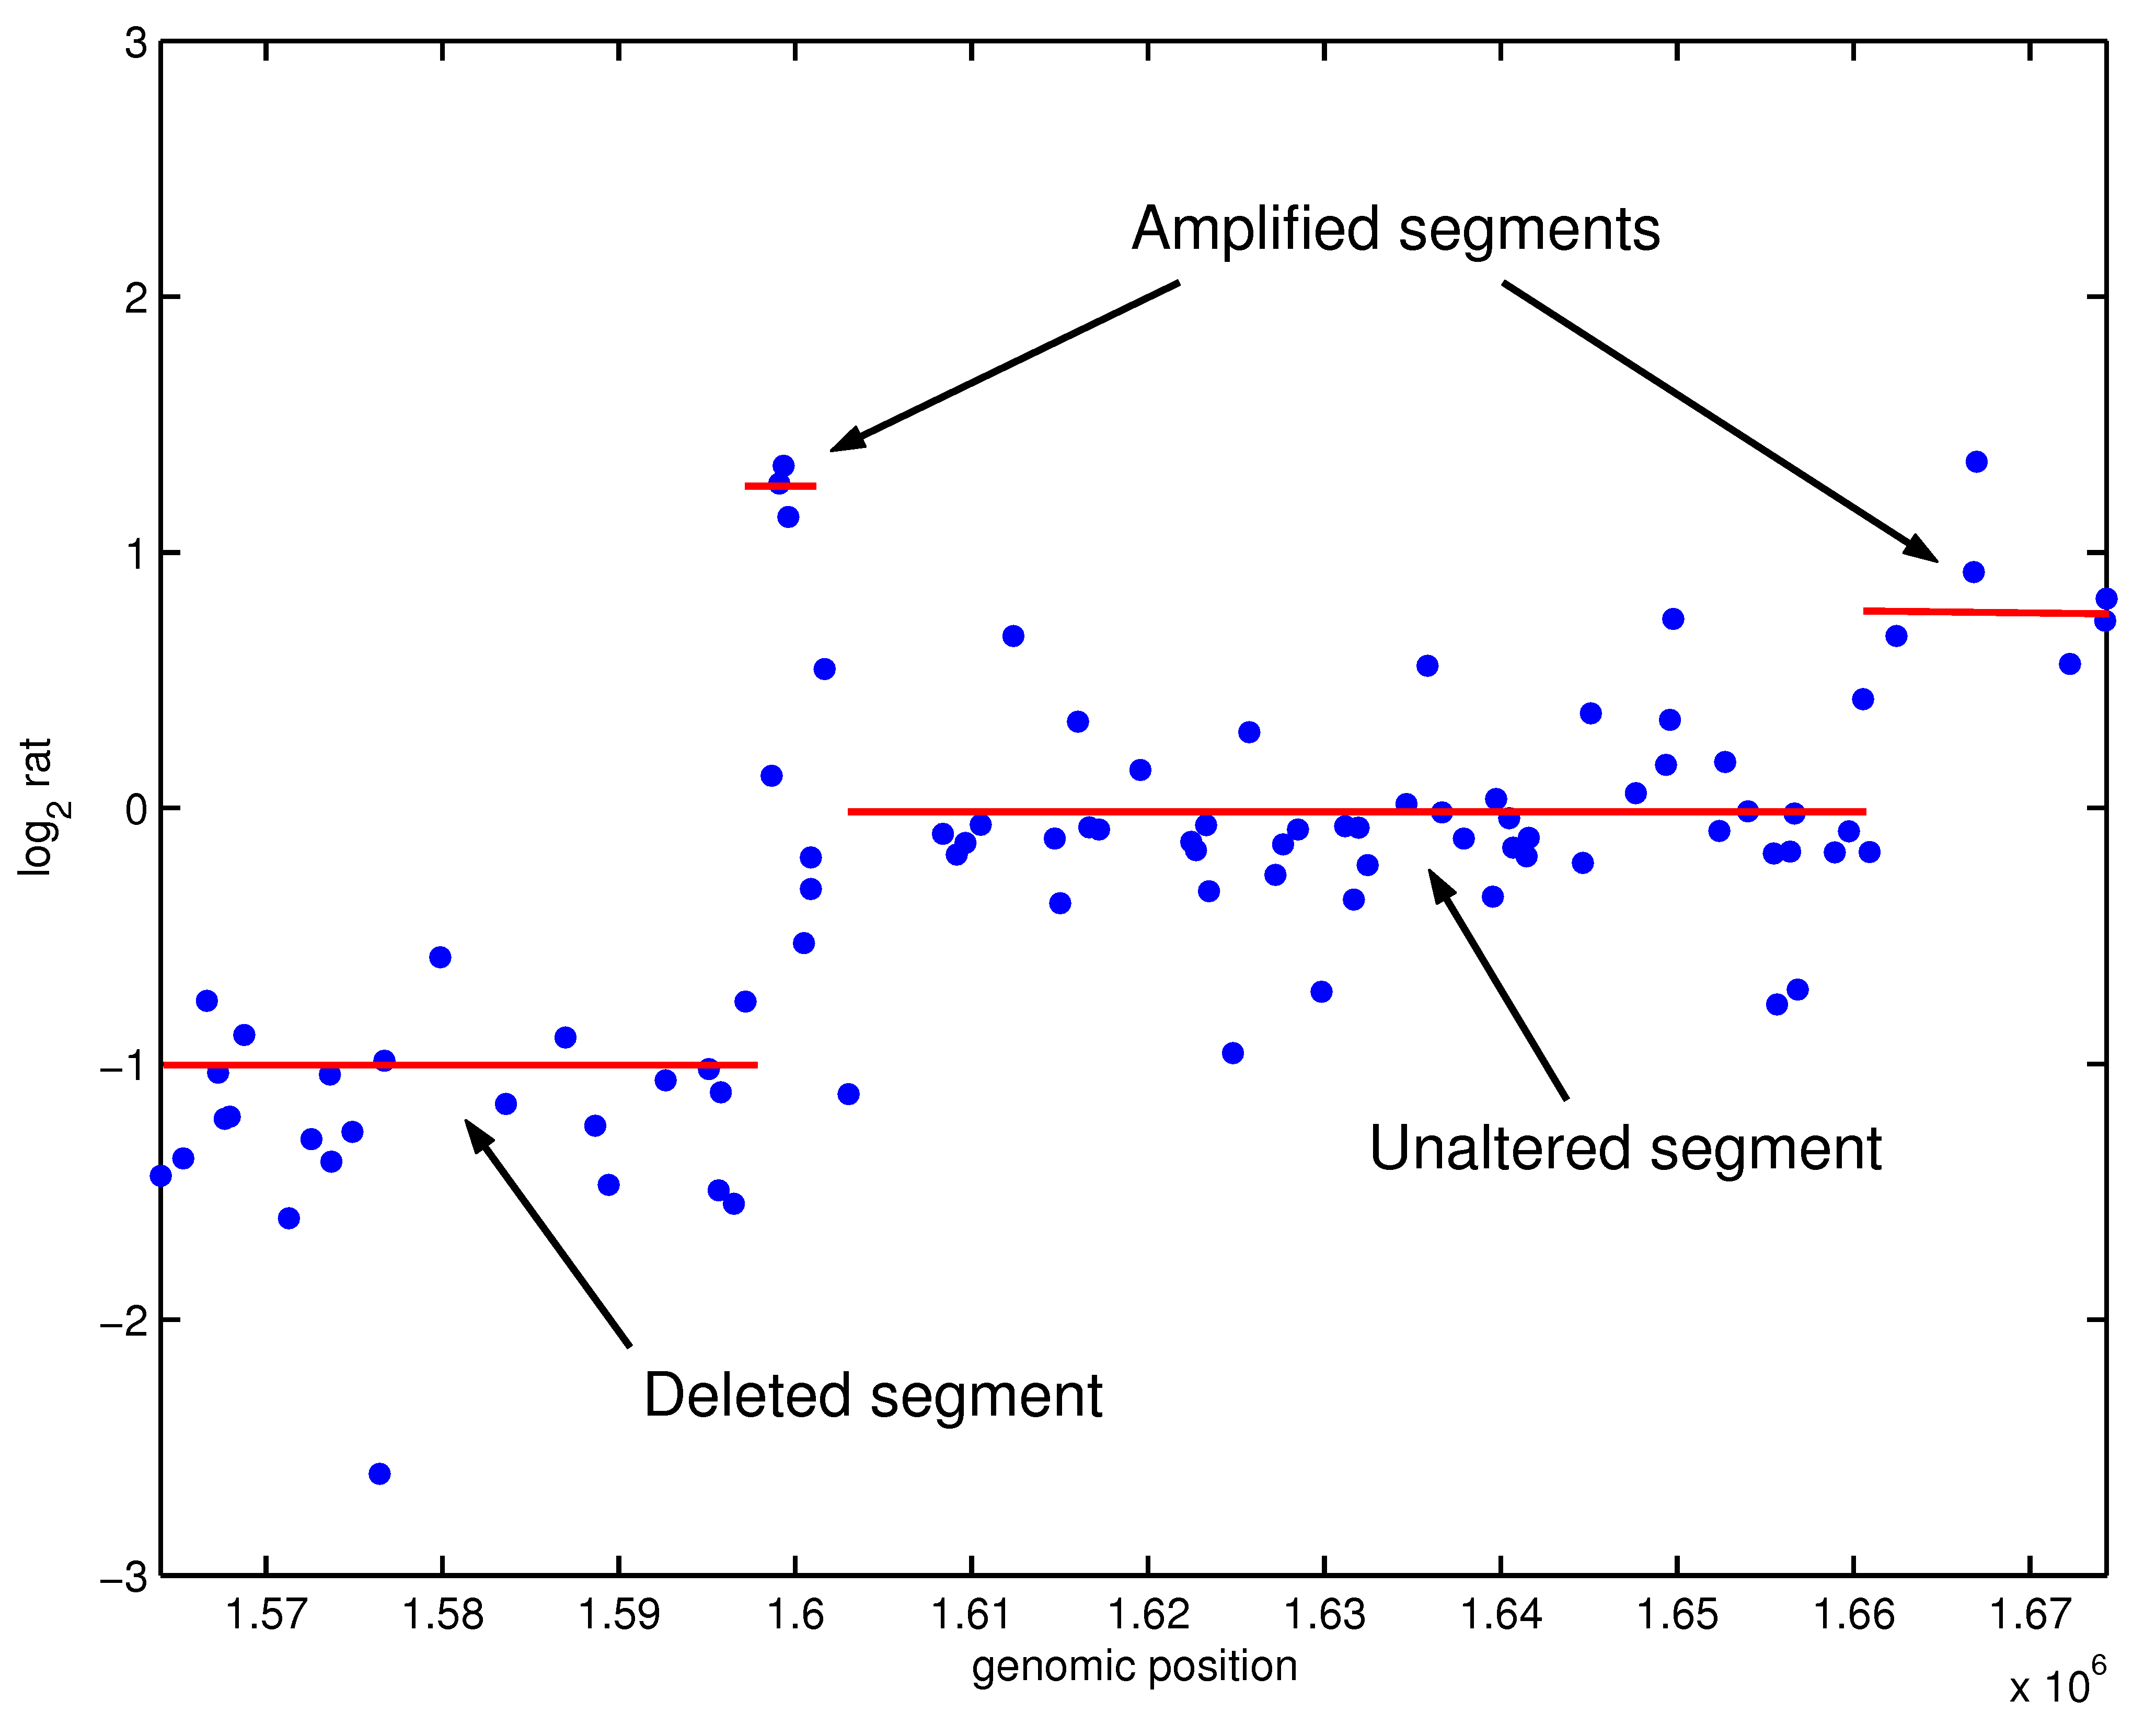
\epsfig{file = /Recherche/CGH/Exposes/Figures/profile_example.eps, clip=,
  bbllx=60, bblly=196, bburx=543, bbury=586}
$$
\centerline{
  A dot on the graph 
  $
  \displaystyle{
    = \log_2 \left\{ \frac{\text{ $\sharp$ copies of BAC(t) in the test
          genome }}{\text{$\sharp$ copies of BAC(t) in the reference
          genome}}\right\}}
  $
}

\paragraph{Interest of clustering: }
Chromosome 1 (obesity):
$$
\begin{tabular}{cc}
  Segmentation & Segmentation/Clustering \\
  $K=2$ & $P=3$, $K=8$ \\
  \epsfig{file = /Recherche/CGH/Exposes/Figures/bt474_c1_seg_hetero_K2.eps, clip=, scale=0.7} 
  & \epsfig{file = /Recherche/CGH/Exposes/Figures/resultat_P3K8.eps , clip=, scale=0.7} 
\end{tabular}
$$
Clustering detects an outliers and captures 'normal' segments within
a large variance region.


%%%%%%%%%%%%%%%%%%%%%%%%%%%%%%%%%%%%%%%%%%%%%%%%%%%%%%%%%%%%%%%%%%%%%%%%
%%%%%%%%%%%%%%%%%%%%%%%%%%%%%%%%%%%%%%%%%%%%%%%%%%%%%%%%%%%%%%%%%%%%%%%%
%%%%%%%%%%%%%%%%%%%%%%%%%%%%%%%%%%%%%%%%%%%%%%%%%%%%%%%%%%%%%%%%%%%%%%%%
%%%%%%%%%%%%%%%%%%%%%%%%%%%%%%%%%%%%%%%%%%%%%%%%%%%%%%%%%%%%%%%%%%%%%%%%
\end{document}
%%%%%%%%%%%%%%%%%%%%%%%%%%%%%%%%%%%%%%%%%%%%%%%%%%%%%%%%%%%%%%%%%%%%%%%%
%%%%%%%%%%%%%%%%%%%%%%%%%%%%%%%%%%%%%%%%%%%%%%%%%%%%%%%%%%%%%%%%%%%%%%%%
%%%%%%%%%%%%%%%%%%%%%%%%%%%%%%%%%%%%%%%%%%%%%%%%%%%%%%%%%%%%%%%%%%%%%%%%
%%%%%%%%%%%%%%%%%%%%%%%%%%%%%%%%%%%%%%%%%%%%%%%%%%%%%%%%%%%%%%%%%%%%%%%%
